\documentclass[spanish,a4paper,11pt,twoside]{report}

%%%%%%%%%%%%%%%%%%%%%%%%%%%%%%%%%%%%%%%%%%%%%%%%%%%%%%%%%%%%%%%%%%%%%%%%%%%%%%%
\usepackage[dvips]{graphicx}
\usepackage[dvips]{epsfig}
\usepackage[latin1]{inputenc}
\usepackage[spanish]{babel}
\usepackage{alltt}
\usepackage{templates/algorithm}
\usepackage{templates/algorithmic}
\usepackage{templates/multirow}

%%%%%%%%%%%%%%%%%%%%%%%%%%%%%%%%%%%%%%%%%%%%%%%%%%%%%%%%%%%%%%%%%%%%%%%%%%%%%%%

\newcommand{\SONY}{{\sc Sony}}
\newcommand{\MICROSOFT}{{\sc Microsoft}}
\newcommand{\GCC}{\textsf{\textsc{G}CC}}
\newcommand{\INTEL}{\textsf{\textsc{I}ntel}}

%%% Traducimos el pseudocodigo
\renewcommand{\algorithmicwhile}{\textbf{mientras}}
\renewcommand{\algorithmicend}{\textbf{fin}}
\renewcommand{\algorithmicdo}{\textbf{hacer}}
\renewcommand{\algorithmicif}{\textbf{si}}
\renewcommand{\algorithmicthen}{\textbf{entonces}}
\renewcommand{\algorithmicrepeat}{\textbf{repetir}}
\renewcommand{\algorithmicuntil}{\textbf{hasta que}}
\renewcommand{\algorithmicelse}{\textbf{en otro caso}}
\renewcommand{\algorithmicfor}{\textbf{para}}

%\newcommand{\RETURN}{\textbf{retornar} }
\newcommand{\RET}{\STATE \textbf{retornar} }
\newcommand{\TO}{\textbf{hasta} }
\newcommand{\AND}{\textbf{y} }
\newcommand{\OR}{\textbf{o} }

%%%%%%%%%%%%%%%%% Creamos un entorno para listar c�digo fuente %%%%%%%%%%%%%%%
\newenvironment{sourcecode}
{\begin{list}{}{\setlength{\leftmargin}{1em}}\item\scriptsize\bfseries}
{\end{list}}

\newenvironment{littlesourcecode}
{\begin{list}{}{\setlength{\leftmargin}{1em}}\item\tiny\bfseries}
{\end{list}}

\newenvironment{summary}
{\par\noindent\begin{center}\textbf{Abstract}\end{center}\begin{itshape}\par\noindent}
{\end{itshape}}

\newenvironment{keywords}
{\begin{list}{}{\setlength{\leftmargin}{1em}}\item[\hskip\labelsep \bfseries Keywords:]}
{\end{list}}

\newenvironment{palabrasClave}
{\begin{list}{}{\setlength{\leftmargin}{1em}}\item[\hskip\labelsep \bfseries Palabras clave:]}
{\end{list}}


%%%%%%%%%%%%%%%%%%%%%%%%%%%%%%%%%%%%%%%%%%%%%%%%%%%%%%%%%%%%%%%%%%%%%%%%%%%%%%%
% Format
%%%%%%%%%%%%%%%%%%%%%%%%%%%%%%%%%%%%%%%%%%%%%%%%%%%%%%%%%%%%%%%%%%%%%%%%%%%%%%%

%%\topmargin -4 mm
%\topmargin -21 mm
%\headheight 10 mm
%\headsep 10 mm

%\textheight 229 mm
%\textheight 246 mm

%\oddsidemargin -5.4 mm
%\evensidemargin -5.4 mm
\oddsidemargin 5 mm
\evensidemargin 5 mm

%\oddsidemargin -3 mm
%\evensidemargin -3 mm

%\textwidth 17 cm
\textwidth 15 cm
%\columnsep 10 mm

\input{amssym.def}

%%%%%%%%%%%%%%%%%%%%%%%%%%%%%%%%%%%%%%%%%%%%%%%%%%%%%%%%%%%%%%%%%%%%%%%%%%%%%%%

\begin{document}

%%%%%%%%%%%%%%%%%%%%%%%%%%%%%%%%%%%%%%%%%%%%%%%%%%%%%%%%%%%%%%%%%%%%%%%%%%%%%%%
% First Page 
%%%%%%%%%%%%%%%%%%%%%%%%%%%%%%%%%%%%%%%%%%%%%%%%%%%%%%%%%%%%%%%%%%%%%%%%%%%%%%%

\pagestyle{empty}
\thispagestyle{empty}


\newcommand{\HRule}{\rule{\linewidth}{1mm}}
\setlength{\parindent}{0mm}
\setlength{\parskip}{0mm}
\vspace*{\stretch{1}}

\begin{center}

\includegraphics[width=0.2\textwidth]{images/logotipo-secundario-ULL}\\[0.25cm]
\end{center}

\HRule
\begin{center}
        {\Huge Bisecci�n de $f(x)=cos($\pi$x)$} \\[2.5mm] 
        {\Huge Informe Cient�fico-T�cnico} \\[2.5mm]
        {\Large Carmen Laura Mart�n Gonz�lez y David T�mas Montesdeoca Flores} \\[5mm]
        {\Large \textit{Grupo ($1\midA$) }} \\[5mm]


        {\em T�cnicas Experimentales. $1^{er}$ curso. $2^{do}$ semestre} \\[5mm]
        Lenguajes y Sistemas Inform�ticos \\[5mm]
        Facultad de Matem�ticas \\[5mm]
        
        Universidad de La Laguna \\
\end{center}
\HRule
\vspace*{\stretch{2}}
\begin{center}
  La Laguna, 11 de Mayo de 2014 
\end{center}

%%%%%%%%%%%%%%%%%%%%%%%%%%%%%%%%%%%%%%%%%%%%%%%%%%%%%%%%%%%%%%%%%%%%%%%%%%%%%%%

%%%%%%%%%%%%%%%%%%%%%%%%%%%%%%%%%%%%%%%%%%%%%%%%%%%%%%%%%%%%%%%%%%%%%%%%%%%%%%%
\newpage{\pagestyle{empty}\cleardoublepage}

\pagestyle{myheadings} %my head defined by markboth or markright
% No funciona bien \markboth sin "twoside" en \documentclass, pero al
% ponerlo se dan un mont�n de errores de underfull \vbox, con lo que no se
% ha puesto.
\markboth{Carmen Laura y David T�mas}{Bisecci�n de $f(x)=cos($\pi$x)$}

%%%%%%%%%%%%%%%%%%%%%%%%%%%%%%%%%%%%%%%%%%%%%%%%%%%%%%%%%%%%%%%%%%%%%%%%%%%%%%%
%Numeracion en romanos
\renewcommand{\thepage}{\roman{page}}
\setcounter{page}{1}

%%%%%%%%%%%%%%%%%%%%%%%%%%%%%%%%%%%%%%%%%%%%%%%%%%%%%%%%%%%%%%%%%%%%%%%%%%%%%%%

\tableofcontents

%%%%%%%%%%%%%%%%%%%%%%%%%%%%%%%%%%%%%%%%%%%%%%%%%%%%%%%%%%%%%%%%%%%%%%%%%%%%%%%
\newpage{\pagestyle{empty}\cleardoublepage}

\listoffigures

%%%%%%%%%%%%%%%%%%%%%%%%%%%%%%%%%%%%%%%%%%%%%%%%%%%%%%%%%%%%%%%%%%%%%%%%%%%%%%%
\newpage{\pagestyle{empty}\cleardoublepage}

\listoftables

%%%%%%%%%%%%%%%%%%%%%%%%%%%%%%%%%%%%%%%%%%%%%%%%%%%%%%%%%%%%%%%%%%%%%%%%%%%%%%%
\newpage{\pagestyle{empty}\cleardoublepage}

%%%%%%%%%%%%%%%%%%%%%%%%%%%%%%%%%%%%%%%%%%%%%%%%%%%%%%%%%%%%%%%%%%%%%%%%%%%%%%%
%Numeracion a partir del capitulo I
\renewcommand{\thepage}{\arabic{page}}
\setcounter{page}{1}

\setlength{\parindent}{5mm}

%%%%%%%%%%%%%%%%%%%%%%%%%%%%%%%%%%%%%%%%%%%%%%%%%%%%%%%%%%%%%%%%%%%%%%%%%%%%%%%
\chapter{Motivaci�n y objetivos}
\label{chapter:obj}

%%%%%%%%%%%%%%%%%%%%%%%%%%%%%%%%%%%%%%%%%%%%%%%%%%%%%%%%%%%%%%%%%%%%%%%%%%%%%
% Chapter 1: Motivaci�n y Objetivos 
%%%%%%%%%%%%%%%%%%%%%%%%%%%%%%%%%%%%%%%%%%%%%%%%%%%%%%%%%%%%%%%%%%%%%%%%%%%%%%%
Este m�todo , que se utiliza para resolver ecuaciones de una variable, est� basado en el "Teorema de los Valores Intermedios" (TVM), en el cual se establece que toda funci�n continua 'f', en un intervalo cerrado $[a,b]$, toma todos los valores que se hallan entre $f(a)$ y $f(b)$, de tal forma que la ecuaci�n $f(x)=0$ tiene una sola ra�z que verifica $f(a)*f(b)<0$.

%---------------------------------------------------------------------------------
\section{�Qu� es el m�todo de bisecci�n?}
\label{1:sec:1}

  El m�todo de la bisecci�n es un algoritmo que nos permite encontrar una ra�z de la funci�n que tengamos. Su funcionamiento es muy similar al de la b�squeda binaria, s�lo que estamos utilizando valores continuos ($\infty$) en lugar de discretos (finitos). Vamos a asumir que las funciones con las que trabajamos son continuas.

  Sabemos que si la funci�n $f(x)$ atraviesa el eje x, en la intersecci�n existe una ra�z, por lo que antes de la ra�z $f(x) > 0$ y despu�s $f(x) < 0$. Entonces, teniendo dos puntos 'a' y 'b' tales que $f(a)$ y $f(b)$ tienen signos opuestos, sabemos que debe haber una ra�z en el intervalo $[a, b]$.

%---------------------------------------------------------------------------------
\section{�C�mo funciona su algoritmo?}
\label{1:sec:2}
  El algoritmo funciona de la siguiente forma: 

\begin{itemize}
  \item Primero tomamos el punto medio entre 'a' y 'b', al cual llamaremos $c ()$. Si el valor de $f(c)=0$, o est� suficientemente cerca.
  \item Segundo tomamos a 'c' como el valor de la ra�z.
\end{itemize}

  En caso contrario:
  
\begin{itemize}
  \item Primero reemplazamos a 'a' o 'b' por 'c', de acuerdo al signo de $f(c)$, de tal forma que los signos de $f(a)$ y $f(b)$ sigan siendo diferentes.
\end{itemize}
  
  Finalmente, repetimos el m�todo con el nuevo intervalo.

%---------------------------------------------------------------------------------
\section{Ventaja del m�todo de bisecci�n.}
\label{1:sec:3}
  
  La principal ventaja de este m�todo es que es muy eficaz aunque menos que el m�todo de Newton, ya que, est� garantizado que el m�todo converge si los valores de $f(a)$ y $f(b)$ son de signos contrarios. La convergencia de este m�todo es lineal, y su error absoluto despu�s de n iteraciones es: $\frac{|b-a|}{2^n}$

%%%%%%%%%%%%%%%%%%%%%%%%%%%%%%%%%%%%%%%%%%%%%%%%%%%%%%%%%%%%%%%%%%%%%%%%%%%%%%%
\chapter{Fundamentos te�ricos}
\label{chapter:teo}

%%%%%%%%%%%%%%%%%%%%%%%%%%%%%%%%%%%%%%%%%%%%%%%%%%%%%%%%%%%%%%%%%%%%%%%%%%%%%%%
% Chapter 2: Fundamentos Te�ricos 
%%%%%%%%%%%%%%%%%%%%%%%%%%%%%%%%%%%%%%%%%%%%%%%%%%%%%%%%%%%%%%%%%%%%%%%%%%%%%%%

%++++++++++++++++++++++++++++++++++++++++++++++++++++++++++++++++++++++++++++++

En este cap�tulo se han de presentar los antecedentes te�ricos y pr�cticos que
apoyan el tema objeto de la investigaci�n.

%++++++++++++++++++++++++++++++++++++++++++++++++++++++++++++++++++++++++++++++

\section{Primer apartado del segundo cap�tulo}
\label{2:sec:1}
  Primer p�rrafo de la primera secci�n.

\section{Segundo apartado del segundo cap�tulo}
\label{2:sec:2}
  Primer p�rrafo de la segunda secci�n.



%%%%%%%%%%%%%%%%%%%%%%%%%%%%%%%%%%%%%%%%%%%%%%%%%%%%%%%%%%%%%%%%%%%%%%%%%%%%%%%
\chapter{Procedimiento experimental}
\label{chapter:exp}

%%%%%%%%%%%%%%%%%%%%%%%%%%%%%%%%%%%%%%%%%%%%%%%%%%%%%%%%%%%%%%%%%%%%%%%%%%%%%%%
% Chapter 3: Procedimiento experimental 
%%%%%%%%%%%%%%%%%%%%%%%%%%%%%%%%%%%%%%%%%%%%%%%%%%%%%%%%%%%%%%%%%%%%%%%%%%%%%%%

Este cap�tulo ha de contar con seccciones para la descripci�n de los experimentos 
y del material.
%
Tambi�n debe haber una secci�n para los resultados obtenidos y una �ltima de 
an�lisis de los resultados.

%++++++++++++++++++++++++++++++++++++++++++++++++++++++++++++++++++++++++++++++
\section{Descripci�n de los experimentos}
\label{3:sec:1}

bla, bla, etc. 

%++++++++++++++++++++++++++++++++++++++++++++++++++++++++++++++++++++++++++++++
\section{Descripci�n del material}
\label{3:sec:2}

('default', 'Feb 27 2014 20:00:17')

Linux-3.2.0-61-generic-i686-with-Ubuntu-12.04-precise

('Linux', 'FISICA-PC', '3.2.0-61-generic', '#93-Ubuntu SMP Fri May 2 21:33:33 UTC 2014', 'i686', 'i686')

2.7.3

Genuine Intel(R) CPU            2160  @ 1.80GHz

GenuineIntel

1200.000 Hz

1024 KB


%++++++++++++++++++++++++++++++++++++++++++++++++++++++++++++++++++++++++++++++
\section{Resultados obtenidos}
\label{3:sec:3}

bla, bla, etc. 


%------------------------------------------------------------------------------
\begin{figure}[!th]
\begin{center}
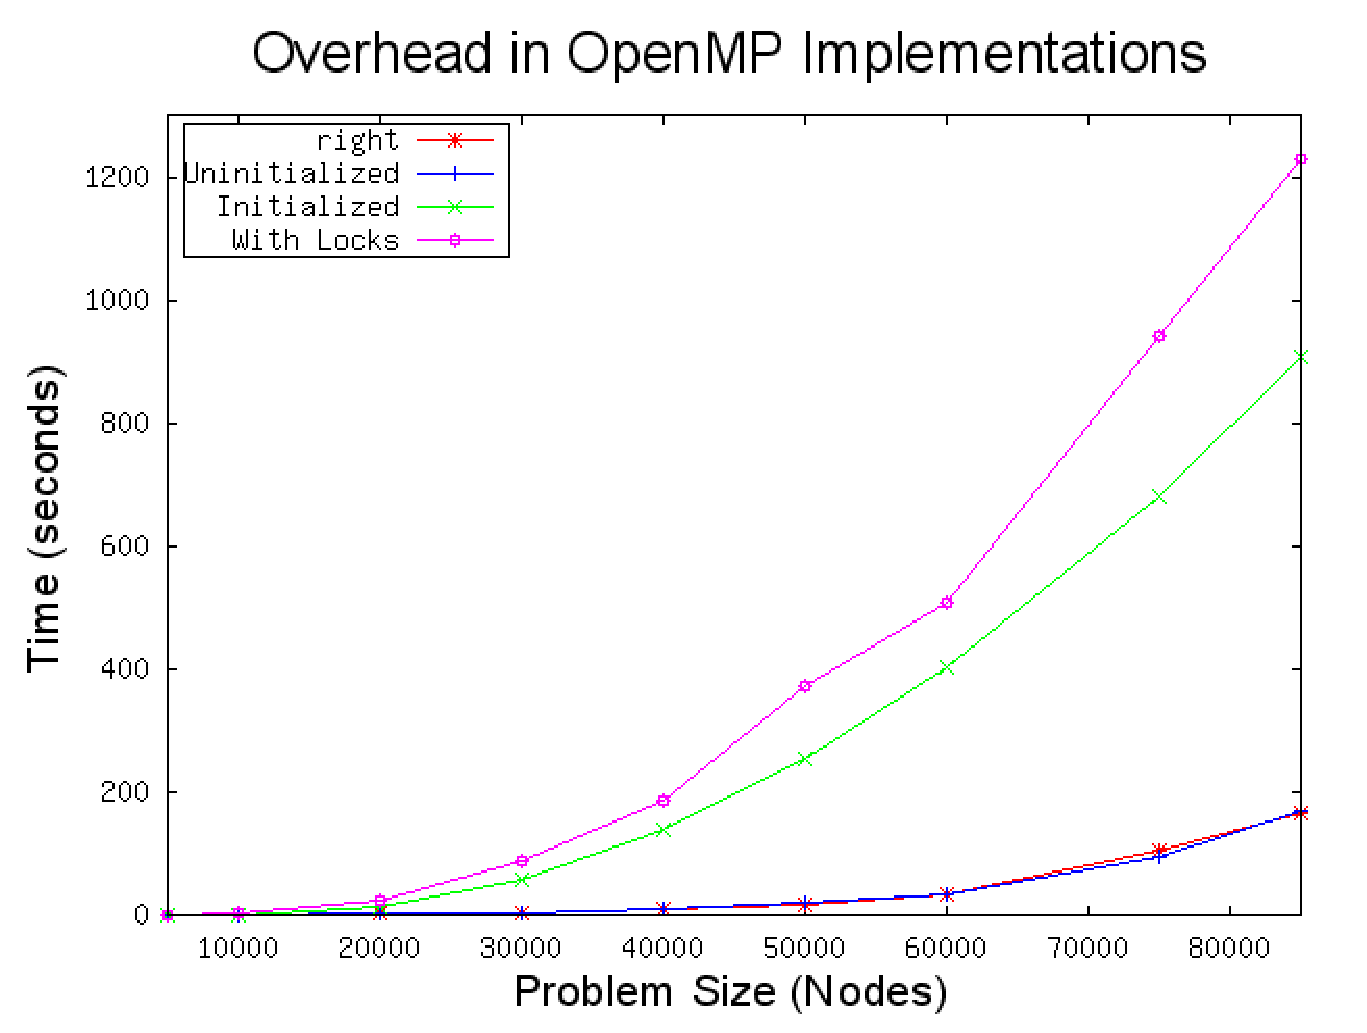
\includegraphics[width=0.75\textwidth]{images/figura1.eps}
\caption{Ejemplo de figura}
\label{fig:1}
\end{center}
\end{figure}
%------------------------------------------------------------------------------
\begin{figure}[!ht]
\begin{center}

\includegraphics[width=0.75\textwidth]{images/imagen1.eps}
\caption{Ejemplo de figura con gr�fico}
\label{fig}
\end {center}
\end {figure}

%------------------------------------------------------------------------------
%--------------------------------------------------------------------------
\begin{table}[!ht]
\begin{center}
\begin{tabular}{|c|c|} \hline 
\textbf{Tiempo  } & \textbf{Velocidad} \\ 
\textbf{($\pm$ 0.001 s)} & \textbf{($\pm$ 0.1 m/s)} \\ \hline \hline
1.234 &
67.8
\\
\hline

2.345 &
78.9
\\
\hline

3.456 &
89.1
\\
\hline

4.567 &
91.2
\\
\hline

\end{tabular}
\end{center}
\caption{Resultados experimentales de tiempo (s) y velocidad (m/s)}
\label{tab:1}
\end{table}


%------------------------------------------------------------------------------

%++++++++++++++++++++++++++++++++++++++++++++++++++++++++++++++++++++++++++++++
\section{An�lisis de los resultados}
\label{3:sec:4}

bla, bla, etc. 



%%%%%%%%%%%%%%%%%%%%%%%%%%%%%%%%%%%%%%%%%%%%%%%%%%%%%%%%%%%%%%%%%%%%%%%%%%%%%%%
\chapter{Conclusiones}
\label{chapter:conclusiones}

%%%%%%%%%%%%%%%%%%%%%%%%%%%%%%%%%%%%%%%%%%%%%%%%%%%%%%%%%%%%%%%%%%%%%%%%%%%%%
% Chapter 4: Conclusiones y Trabajos Futuros 
%%%%%%%%%%%%%%%%%%%%%%%%%%%%%%%%%%%%%%%%%%%%%%%%%%%%%%%%%%%%%%%%%%%%%%%%%%%%%

Para concluir tenemos que mencionar varios puntos del trabajo:

\begin{itemize}

\item \textsf{Python} esta en movimiento y en pleno desarrollo, pera ya es una realidad y una interesante opcion para realizar todo tipo de programas que se ejecuten en cualquier maquina. El equipo de desarrollo esta trabajando de manera cada vez mas organizada y cuentan con el apoyo de una comunidad que esta creciendo rapidamente.

\item Algunas de las ventajas que tiene \LaTeX{} son que, crea con facilidad estructuras complejas como pies de pagina, indices, tablas, etc, y para la rama de ciencias tiene principalmente una ventaja primordial que es que se pueden crear con facilidad formulas matematicas.

\item \textsc{Beamer} tiene todas las ventajas de \LaTeX{}. Su presentacion en PDF es estandar y portable. Ademas tiene unos estilos predefinidos con botones de navegacion, tablas de contenidos, pies de pagina informativos, etc.


\item El metodo de la Biseccion converge lentamente, lo que genera la propagacion de error por la cantidad de operaciones e iteraciones necesarias para que el metodo converja.

\end{itemize}

Finalmente, al complementar los elementos mencionados anteriormente y centrandonos en el calculo de las raices mediante el metodo de biseccion, hemos aprendido a crear un fichero de texto y una presentacion a modo de diapositivas, con un cierto grado de exigencia. Tambien hemos aprendido a ser independientes buscando la informacion correcta sobre el tema propuesto y a la vez aprender a trabajar en equipo.
Bajo nuestro punto de vista este es el objetivo de la programacion de este trabajo, ya que, esto nos serviria para los trabajos futuros que tengamos que realizar.

%%%%%%%%%%%%%%%%%%%%%%%%%%%%%%%%%%%%%%%%%%%%%%%%%%%%%%%%%%%%%%%%%%%%%%%%%%%%%%%

%%%%%%%%%%%%%%%%%%%%%%%%%%%%%%%%%%%%%%%%%%%%%%%%%%%%%%%%%%%%%%%%%%%%%%%%%%%%%%%
\newpage{\pagestyle{empty}\cleardoublepage}
\thispagestyle{empty}
\begin{appendix}

\chapter{T�tulo del Ap�ndice 1}
\label{appendix:1}

\section{Algoritmo XXX}
\label{Apendice1:XXX}

\begin{center}
\begin{footnotesize}
\begin{verbatim}
###################################################################################
# Fichero .py
###################################################################################
#
# AUTORES
#   
# FECHA
#
# DESCRIPCION
#
###################################################################################
\end{verbatim}
\end{footnotesize}
\end{center}

\section{Algoritmo YYY}
\label{Apendice1:YYY}

\begin{center}
\begin{footnotesize}
\begin{verbatim}
/###################################################################################
 # Fichero .h
 ###################################################################################
 #
 # AUTORES
 #
 # FECHA
 #
 # DESCRIPCION
 #
 ##################################################################################
\end{verbatim}
\end{footnotesize}
\end{center}


\chapter{T�tulo del Ap�ndice 2}
\label{appendix:2}

\section{Explicacion del codigo \textsf{Python} }
\label{Apendice2:label}

Como dijimos en el apendice anterior, se trata del codigo de un programa realizado en python para calcular la biseccion de f(x)=Cos($\pi$x)  en un intervalo introducido por el usuario junto con el margen de error. ademas calcula el tiempo de ejecucion y dibuja la grafica en otro intervalo que desee el usuario.\par

Primero importamos las librerias necesarias. En este caso las necesitamos para calcular el tiempo, para las funciones trigonometricas (Coseno), y para representar graficas.

\begin{verbatim}
#! /usr/bin/python
#!encoding: UTF-8
import time
import math
import matplotlib.pyplot as pl
import numpy as np
import sys
\end{verbatim}

Definimos las dos funciones que vamos a usar principalmente, una para calcular los valores de f(x) al sustituir un x en ella, y otra para calcular la biseccion.

\begin{verbatim}
def f(x):
  return (math.cos(x*math.pi))
  
def biseccion(a,b,e):
  c=(a+b)/2.0
  while((f(c)!=0.00000001) and (abs(b-a)>e)):
    if f(a)*f(c)<0.00000001:
      b=c
    else:
      a=c
    c=(a+b)/2.0
  return c
\end{verbatim}

A continuacion pedimos al usuario que ingrese los extremos superior e inferior del intervalo y la tolerancia o margen de error.
Establecemos una condicion para poder realizar la biseccion, y es que exista un cambio de signo entre f(A) y f(B), asi que f(A)*f(B)<0. Cuando esto se cumple el programa se ejecuta, empezando a contar el tiempo y parando este "cronometro" despues del calculo.


\begin{verbatim}
A=float(raw_input("Introduzca el extremo inferior del intervalo (a) en el que se desea buscar la raiz: "))
B=float(raw_input("Introduzca el extremo superior del intervalo (b) en el que se desea buscar la raiz: "))
E=float(raw_input("Introduzca el margen de error a partir del cual no afecte demasiado a sus calculos: "))
if f(A)*f(B)<0.00000001:
  start=time.time()
  r=biseccion(A,B,E)
  finish=time.time()-start
  print "La raiz que se ha calculado en ese intervalo de forma aproximada es:%4.3f" %r
  print "El tiempo que ha tardado en ejecutarse el calculo en segundos es:"
  print finish
  
else:
  print "No podemos asegurar que en el intervalo introducido exista raiz, lo sentimos."
\end{verbatim}


Tras hallar la biseccion deseada, se pide al usuario un valor de x para representar la funcion en un intervalo de -x a x. Con la ayuda de un bucle for conseguimos dar valores desde el 0 hasta x y guardarlos en un vector en los valores de y. De este modo podemos tener los puntos a representar.

\begin{verbatim}
x=int(raw_input("Introduzca el maximo valor de x para la representacion: "))
lista=[]
for i in range(x):
  y=math.cos(math.pi*i)
  lista.append(y)
\end{verbatim}

Por ultimo representamos la funcion. Elejimos el color y el ancho de la linea. Como nos interesa ver el corte con el eje de abcisas, representamos una recta x multiplicada por 0, asi todos sus puntos valdran 0. Le ponemos un titulo a la grafica, la guardamos y la mostramos. 
\begin{verbatim}
pl.figure(figsize=(8,6), dpi=80)

X = np.linspace(-x, x, 256, endpoint=True)
C = np.cos(X*np.pi)
S = 0*(X)

pl.plot(X,C, color="cyan", linewidth=2.5, linestyle="-", label="Coseno")
pl.plot(X,S, color="black", linewidth=1.5, linestyle="-", label="Eje X")
pl.legend(loc='upper left')
pl.xlim(X.min()*1.1,X.max()*1.1)
pl.ylim(C.min()*1.1,C.max()*1.1)
pl.yticks([-1, 0, +1])
pl.title("Representacion grafica")
pl.savefig("cos.eps", dpi=72)
\end{verbatim}

Y aqui termina el codigo.

\end{appendix}

%%%%%%%%%%%%%%%%%%%%%%%%%%%%%%%%%%%%%%%%%%%%%%%%%%%%%%%%%%%%%%%%%%%%%%%%%%%%%%%
\addcontentsline{toc}{chapter}{Bibliograf�a}
\bibliographystyle{plain}


\bibliography{bib/references}
\nocite{*}

%%%%%%%%%%%%%%%%%%%%%%%%%%%%%%%%%%%%%%%%%%%%%%%%%%%%%%%%%%%%%%%%%%%%%%%%%%%%%%%

\end{document}
